\documentclass{article}

% Language setting
% Replace `english' with e.g. `spanish' to change the document language
\usepackage[spanish]{babel}

% Set page size and margins
% Replace `letterpaper' with `a4paper' for UK/EU standard size
\usepackage[letterpaper,top=2cm,bottom=2cm,left=3cm,right=3cm,marginparwidth=1.75cm]{geometry}


% Useful packages
\usepackage{amsthm}
\usepackage{amssymb}
\PassOptionsToPackage{normalem}{ulem}
\usepackage{ulem}
\usepackage[T1]{fontenc}
\usepackage{float}
\usepackage{xmpmulti}
\usepackage{algorithm,algpseudocode}
\usepackage{amsmath}
\usepackage{graphicx}
\usepackage{tabularx}
\usepackage[colorlinks=true, allcolors=blue]{hyperref}

\title{Análisis del algoritmo de ordenamiento de Timsort}
\author{Samy Felipe Cuestas Merchan, Camilo Hernández Guerrero, Juan Camilo Mendieta Hernández}

\begin{document}
\maketitle

\begin{abstract}
En este documento se presenta el análisis del ordenamiento de TimSort. Los elementos a presentar son análisis, diseño y algoritmo de Timsort.
\end{abstract}

\section{Parte I: Análisis y diseño del algoritmo}
\subsection{Análisis}

El problema parte de la necesidad de ordenar una secuencia dada mediante el uso del algoritmo de ordenamiento conocido como Timsort, dicha secuencia está dada por
\[
S=\left\langle s_{1},s_{2},\cdots,s_{n}\right\rangle =\left\langle s_{i}\in\mathbb{Z}\land1\le i\le n\right\rangle 
\]
donde S es la secuencia entrante, n es el tamaño de la secuencia, i es el índice de cada elemento y $\mathbb{Z}$ es el conjunto de los números enteros.
\subsection{Diseño}

\subsubsection{Entradas}

Como entradas tenemos la secuencia $S = \left\langle s_{i}\in\mathbb{T}\land1\le i\le n\right\rangle $ de $n\in\mathbb{N}$ elementos que pertenecen a un conjunto $\mathbb{T}$. 
\subsubsection{Salidas}

Como salidas tenemos la secuencia $S = \left\langle s_{i}\in\mathbb{T}\land1\le i\le n\right\rangle $ pero con sus elementos cumpliendo la relacion de orden parcial $\leq$ para cada elemento adyacente.

\section{Parte II: Algoritmos}




\subsection{Timsort}

\begin{algorithm}[H]
\begin{algorithmic}[1]
\Procedure{TimSort}{$S$}
  \State$minRun\leftarrow calcMinRun(|S|)$
  \For{$i\leftarrow0$ \textbf{to} $\left|S\right| \textbf{of tam } minRun$}
    \State$end\leftarrow$ \textsc{min(i + minRun - 1, n - 1)}
    \State\textsc{InsertionSort(S, i, end)}
  \EndFor
  \State$size\leftarrow minRun$ 
  \While{$size < n$}
    \For{$left\leftarrow0$ \textbf{to} $\left|S\right| \textbf{of tam } 2 * size$}
        \State$mid\leftarrow$\textsc{min(n - 1, left + size - 1)}
        \State$right\leftarrow$\textsc{min(left + 2 * size - 1, n - 1)}
        \If{$mid < right$}
        \State\textsc{merge(S, left, mid, right)}
        \EndIf
    \EndFor
    \State$size\leftarrow2 * size$ 
    \EndWhile
\EndProcedure
\end{algorithmic}


\caption{Ordenamiento TimSort}
\end{algorithm}


\subsection{Calculo del run minimo}

\begin{algorithm}[H]
\begin{algorithmic}[1]
\Procedure{calcMinRun}{$|S|$}
  \State$r\leftarrow 0$
  \While{$n >= 32$}
    \State$r  \textbf{$ |{}$} \leftarrow n \And1$
    \State$r  \textbf{$ >{}>$} \leftarrow1$
    \EndWhile
    \State\Return {$n + r$}
\EndProcedure
\end{algorithmic}
\caption{calcMinRun}
\end{algorithm}

\subsection{Mezcla de subsecuencias}
\begin{algorithm}[H]
\begin{algorithmic}[1]
\Procedure{Merge}{$S, l, m, r$}

  \State$len1\leftarrow m - l + 1$
  \State$len2\leftarrow r - m$

  \For {$i \leftarrow 0 $  \textbf{to} $\left len1 \right$}

    \State$left$ \textbf{append} $S[l + i]$

  \EndFor
  \For {$i \leftarrow 0 $  \textbf{to} $\left len2 \right$}

    \State$right$ \textbf{append} $S[m + 1 + i]$

  \EndFor
  \State$i\leftarrow 0$
  \State$j\leftarrow 0$
  \State$k\leftarrow l$
  \While{$i < len1$ \textbf{and} $j < len2$}
    \If{$left [i] \leq right[j]$}
        \State$S[k] \leftarrow left[i]$
        \State$i \leftarrow i + 1$
    \Else
        \State$S[k] \leftarrow right[j]$
        \State$j \leftarrow j + 1$
    \EndElse
    \EndIf
    \State$k \leftarrow k + 1$
  \EndWhile
  \While{$i < len1$}
    \State$S[k] \leftarrow left[i]$
    \State$k \leftarrow k + 1$
    \State$i \leftarrow i + 1$
  \EndWhile
  \While{$j < len2$}
    \State$S[k] = right[j]$
    \State$k \leftarrow k + 1$
    \State$j \leftarrow j + 1$
  \EndWhile

\EndProcedure

\end{algorithmic}

\caption{Función merge}
\end{algorithm}

\subsection{Ordenamiento por inserción}

\begin{algorithm}[H]
\begin{algorithmic}[1]

\Procedure{InsertionSort}{$S, left, right$}
    \For {$i \leftarrow left + 1 $  \textbf{to} $\left right + 1 \right$}

    \State$j \leftarrow i$
    \While{$j > left$ \textbf{and} $S[j] < S[j - 1]$}
        \State$S[j] \leftarrow S [j - 1]$
        \State$S[j - 1] \leftarrow S [j]$
        \State $j \leftarrow j - 1$
    \EndWhile

  \EndFor
  

\EndProcedure

\end{algorithmic}

\caption{Ordenamiento por inserción}
\end{algorithm}

\subsection{Complejidad}
Por investigación se encontro que el algoritmo TimSort tiene orden de complejidad $O\left(\left|S\right|log(\left|S\right|)\right)$ en su caso promedio y en su peor caso, mientras que en su mejor caso tiene orden de complejidad $\Omega\left\left \right(\left n\right)\right$. Esto gracias a que aprovecha las secciones d ela secuencias que ya están ordenadas para copiarlas directamente en una sebsecuencia sin tener que ordenarlas de nuevo.

\subsection{Invariante}

\begin{itemize}
    \item \textbf{TimSort}Por cada iteración  cada subsecuencia cuyo tamaño se determina por el tamaño de la minima subsecuencia se encuentra organizada, luego se mezcla dando como resultado una secuencia que cumple con la relación de orden parcial <= . 
        \subitem \textbf{Inicio:} La secuencia S esta dividida en i subsecuencias las cuales pueden estar ordenadas y cuyo tamaño es determinado por minrun
        \subitem \textbf{Avance:} En la i-esima permutación la i-esima subsecuencia está ordenada  mientras que en cada iteración del while se mezclan estas subsecuencias 
        \subitem \textbf{Terminación:} S’ es una secuencia ordenada
    \item \textbf{Merge} Las banderas de control $len1$ y $len2$ indican si las variables 
        $i$ y $j$ siguen la relación de orden parcial <.
        \subitem \textbf{Inicio:} Se inicia con el resultado de \textsc{calcMinRun}, dicha función determina la mínima longitud de un run entre 32 y 64 para que el tamaño del arreglo sea menor o igual a una potencia de 2.
        \subitem \textbf{Avance:} Se valida que la variable $size$ sea menor a $n$, de ser así, se elije un punto en el subarreglo para después fusionar el arreglo a su izquierda, el siguiente a este y después se multiplica en 2.
        \subitem \textbf{Terminación:} La variable $size$ es mayor que el tamaño del arreglo.
    \item \textbf{InsertionSort}Por cada iteración  los primeros i elementos están ordenados 
        \subitem \textbf{Inicio:} El elemento i está ordenado.
        \subitem \textbf{Avance:} Por cada iteración los elementos desde el inicio de arreglo hasta i están ordenados.
        \subitem \textbf{Terminación:} S’ es una secuencia ordenada.
\end{itemize}

\section{Reporte de pruebas}
\subsection{Tiempo de ejecución por cantidad de elementos en la secuencia}
En el siguiente gráfico se puede observar la tendencia en el tiempo (en milisegundos) que existe al aumentar la cantidad de elementos existentes en la secuencia S.
	\begin{figure}[H]
        \centering
        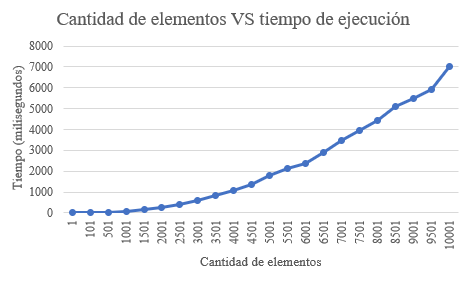
\includegraphics[width=0.7\textwidth]{imagenes/graficoCantidadElementosVSTiempoEjecucion.PNG}
        \caption{Cantidad de elementos VS Tiempo de ejecución}
        \label{fig:ger}
    \end{figure}
    
\subsection{Tabla de los resultados obtenidos}
La siguiente tabla ilustra de manera ordenada y más específica la relación dada en la gráfica de la subsección anterior.
    \begin{center}
    \begin{tabularx}{0.8\textwidth} { 
    | >{\raggedright\arraybackslash}X 
    | >{\centering\arraybackslash}X 
    | >{\raggedleft\arraybackslash}X | }
    \hline
    Tiempo (milisegundos) (y) & Elementos (x) \\
    \hline
    0.004 & 1 \\
    \hline
        \hline
    0.674 & 101  \\
    \hline
        \hline
    17.677 & 501 \\
    \hline
        \hline
    65.881 & 1001 \\
    \hline
        \hline
    153.125 & 1501 \\
    \hline
        \hline
    279.578 & 2001 \\
    \hline
        \hline
    417.878 & 2501 \\
    \hline
        \hline
    608.01 & 3001 \\
    \hline
        \hline
    834.625 & 3501 \\
    \hline
        \hline
    1054.222 & 4001 \\
    \hline
        \hline
    1379.562 & 4501 \\
    \hline
        \hline
    1801.025 & 5001 \\
    \hline
        \hline
    2114.694 & 5501 \\
    \hline
        \hline
    2365.756 & 6001 \\
    \hline
        \hline
    2885.292 & 6501 \\
    \hline
        \hline
    3484.229 & 7001 \\
    \hline
        \hline
    3939.506 & 7501 \\
    \hline
        \hline
    4455.509 & 8001 \\
    \hline
        \hline
    5082.716 & 8501 \\
    \hline
        \hline
    5495.812 & 9001 \\
    \hline
        \hline
    5906.145 & 9501 \\
    \hline
            \hline
    7013.926 & 10001 \\
    \hline
    
    \end{tabularx}
    
    \end{center}
    

\bibliography{sample}
\begin{thebibliography}{0}
  \bibitem{Timsort GeeksforGeeks}  Kumar,A.(26 de junio de 2021) GeeksforGeeks.Recuperado de \url{https://www.geeksforgeeks.org/timsort/}.
  \bibitem{libro guia} Thomas, H., Charles, E., Ronald, L., Clifford, S.(2009).Introduction to Algorithms.Massachusetts,USA: The MIT Press
  \bibitem{video}  Hoque,T.(4 de junio de 2019) Youtube.Recuperado de \url{https://www.youtube.com/watch?v=_dlzWEJoU7I}.
\end{thebibliography}

\end{document}